% Indicate the main file. Must go at the beginning of the file.
% !TEX root = ../main.tex

\chapter{Architecture and Design} % Main chapter title
\label{Chapter2}

\section{Overview of Test Environment}

The test environment consists of a Kubernetes cluster deployed on three bare-metal servers housed in a university datacenter. The three servers are identical in hardware specifications and connected through both a private network and the university network. The setup allows complete remote management and ensures direct communication between the servers for Kubernetes workloads. Below is a detailed description of the hardware and network topology. A diagram illustrating the architecture and network setup is provided in figure~\ref{fig:physical_and_network_infra}.

\begin{figure}[ht]
    \centering
    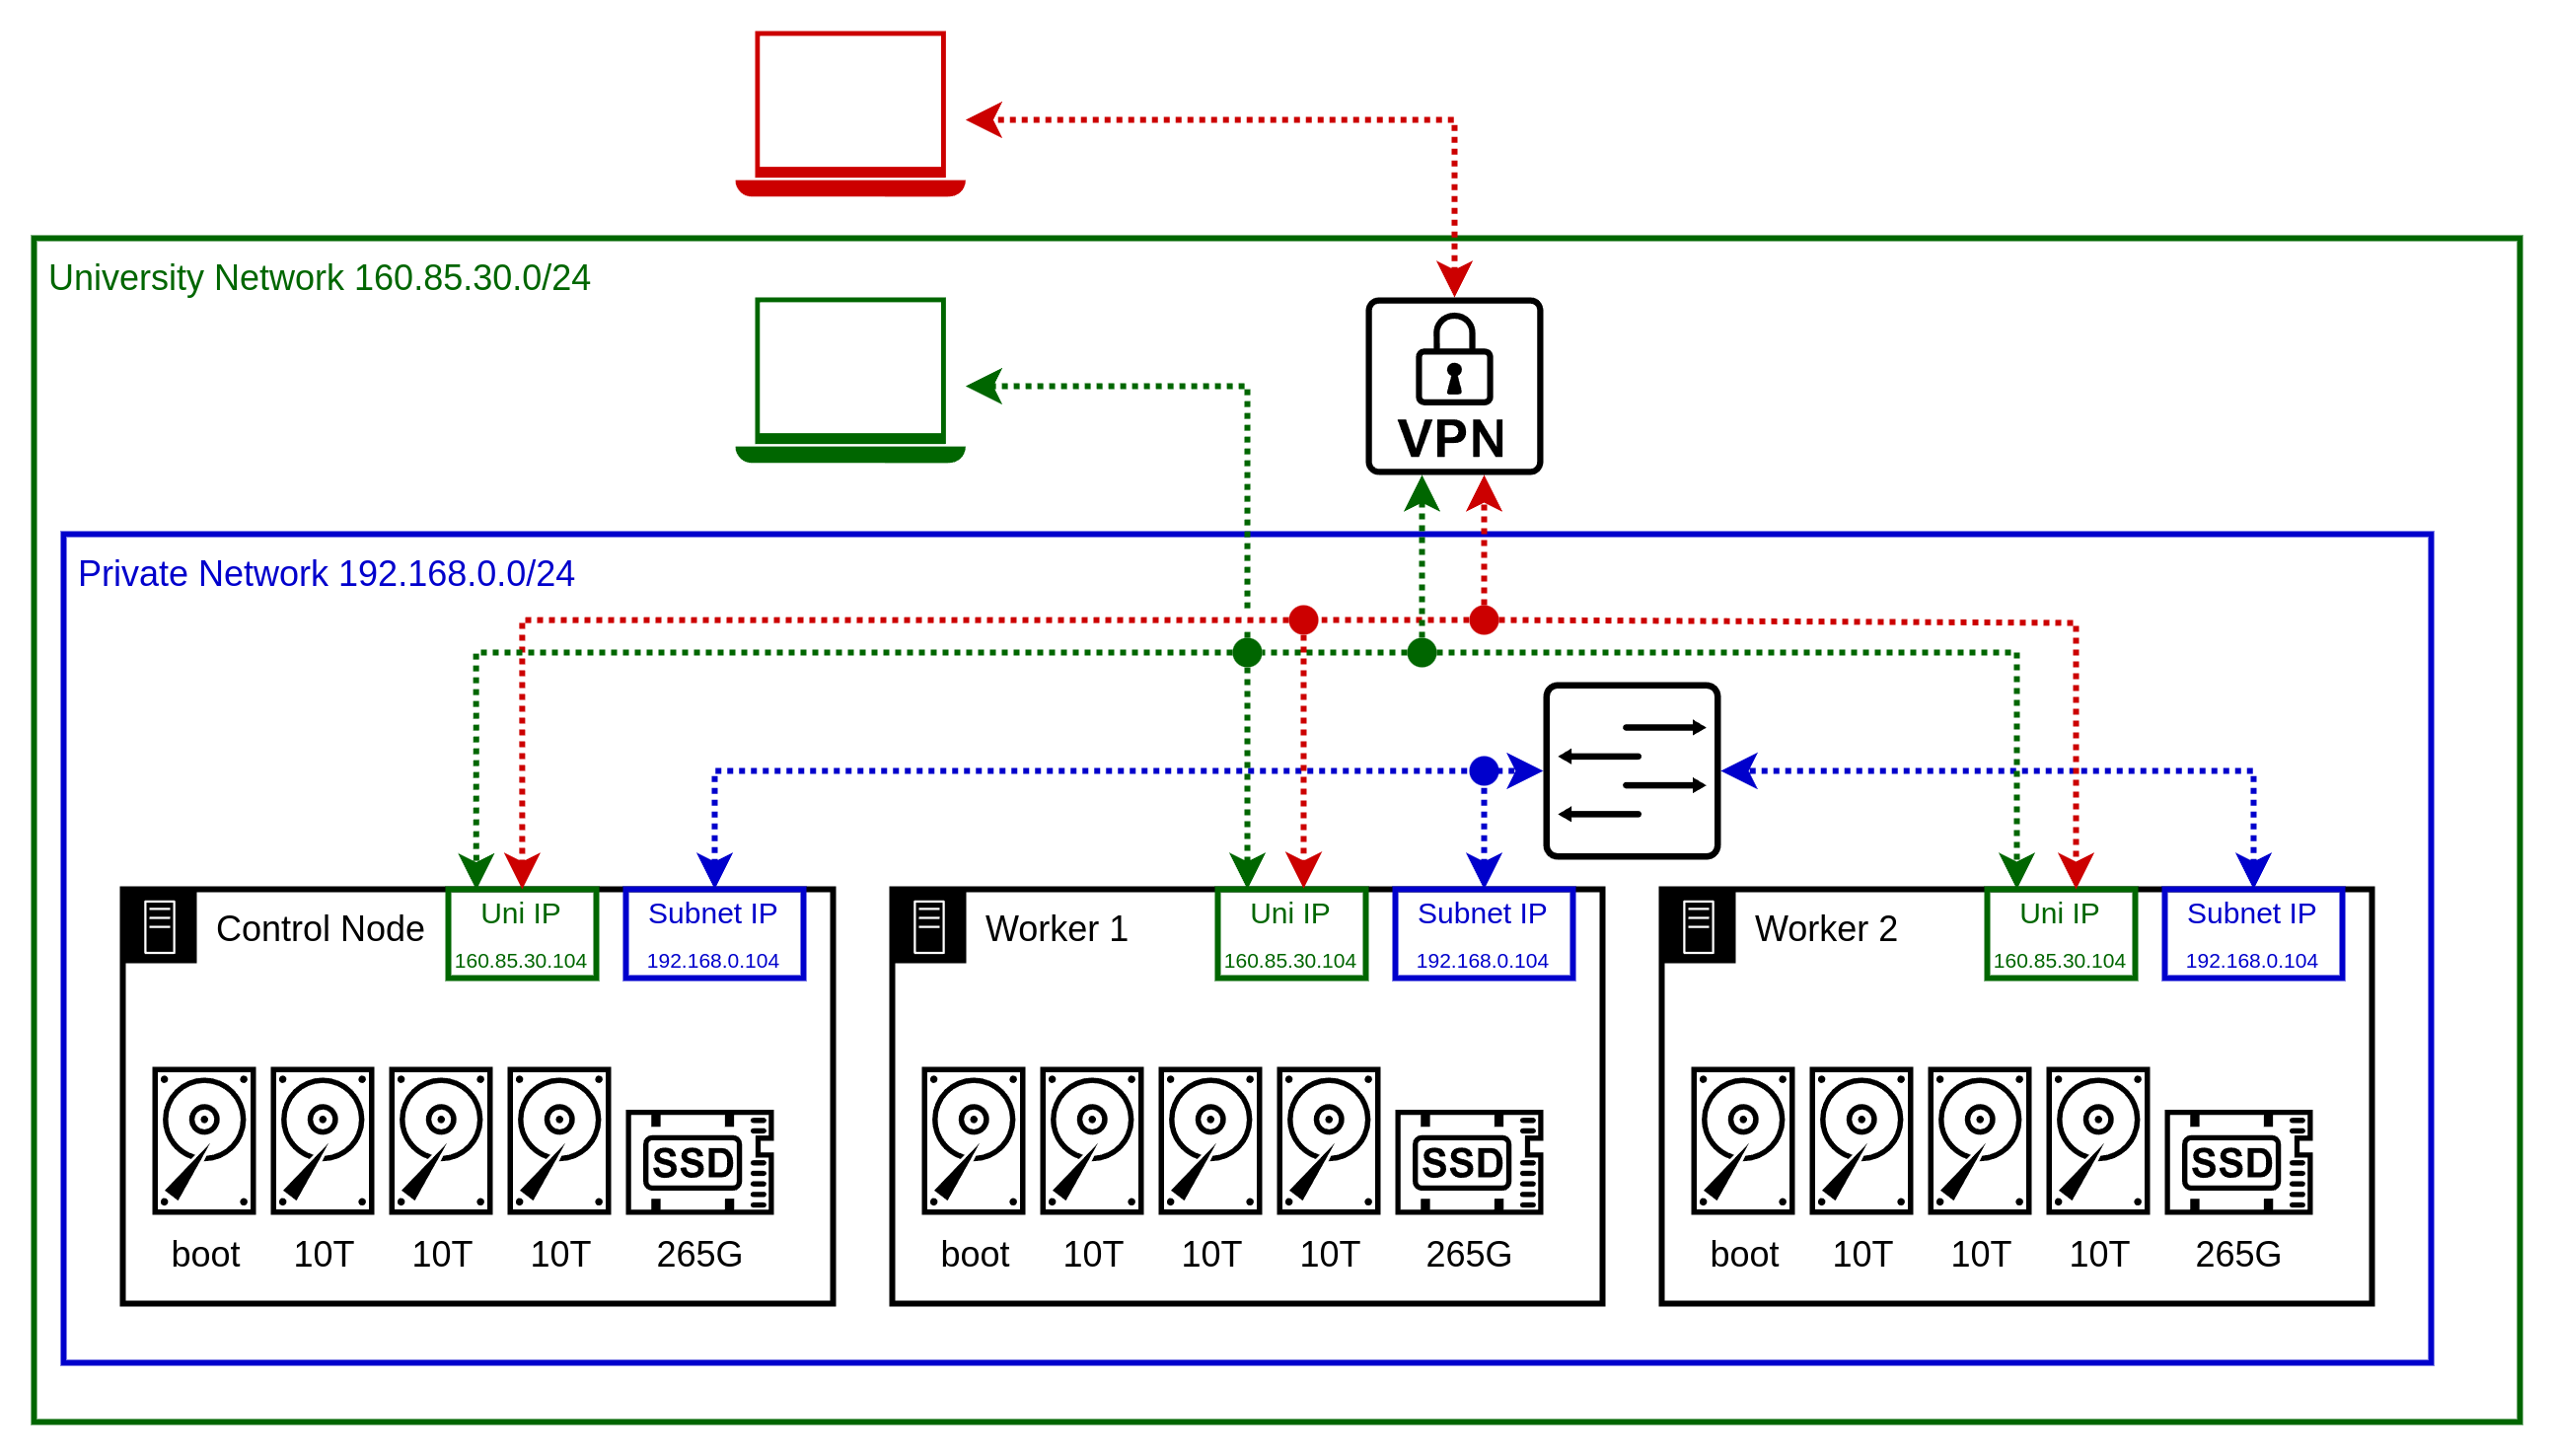
\includegraphics[width=0.9\textwidth]{Figures/physical_and_network_infra.png}
    \decoRule
    \caption[Physical Infrastructure Diagram]{Physical Infrastructure Diagram}
    \label{fig:physical_and_network_infra}
    \end{figure}

\subsection{Hardware and Network}

\subsubsection{Bare-Metal Servers}

The cluster is built using three identical Lenovo ThinkSystem SR530 servers, each equipped with the following hardware:

\begin{itemize}
\item CPU: 1x Intel(R) Xeon(R) Bronze 3104 @ 1.70GHz, 6 cores.
\item Memory: 4x 16GB DDR4 DIMMs, totaling 64GB of RAM per server.
\item Storage:
\begin{itemize}
\item 2x 32GB M.2 SATA SSD for the operating system boot drive.
\item 1x 240GB 6Gbps SATA 2.5" SSD for persistent storage.
\item 3x 10TB 7.2K RPM 12Gbps SAS 3.5" HDDs for bulk storage.
\end{itemize}
\item Power Supply: Dual redundant power supplies.
\item Cooling: 4 out of 6 possible fans installed.
\item Firmware:
\begin{itemize}
\item BMC Version: 8.88 (Build ID: CDI3A4A)
\item UEFI Version: 3.42 (Build ID: TEE180J)
\item LXPM Version: 2.08 (Build ID: PDL142H)
\end{itemize}
\end{itemize}

The servers are equipped with Lenovo XClarity Controller (BMC) for remote management. Each server can be accessed via its BMC IP address for out-of-band management and monitoring.

\subsubsection{Network Topology}

The servers are connected using two distinct networks:

\begin{itemize}
\item Private Network: Each server has a private IP address (192.168.0.104–192.168.0.106), allowing direct, high-speed communication between nodes. This reduces the load on the university network and improves Kubernetes workload performance.
\item University Network: Public-facing IP addresses (160.85.30.104–160.85.30.106) allow access within the university network, with external access enabled via VPN.
\end{itemize}

\textbf{Note}: Detailed switch and gateway configurations are managed by the university IT department and are beyond the scope of this document.
%\subsection{Ubuntu Linux for bare-metal Kubernetes}
%\subsubsection{OS version and Kernel features}
%\subsubsection{Kernel tuning for performance monitoring}

\section{Key Technologies}

\subsection{Ubuntu}
Ubuntu was chosen as the operating system for this project primarily due to the author's familiarity with it. Additionally, it was already installed on the servers when they were received, which saved time and reduced setup complexity. While there are other Linux distributions specifically designed for Kubernetes, using a familiar distribution ensured smoother initial configuration and operation.

\subsection{Bare-Metal K3s}
Installing Kubernetes directly on bare-metal servers (without using a hypervisor or virtual machines) was a fundamental decision to ensure direct access to hardware-level data. This approach allows Kubernetes to interact with the underlying hardware more effectively, which is critical for accurate energy consumption monitoring.

K3s was chosen for several reasons:
\begin{itemize}
\item It is lightweight, making it suitable even for weaker servers, while potentially also lowering energy consumption.
\item Despite its lightweight nature, it remains fully compatible with stock Kubernetes, ensuring that standard Kubernetes resources and configurations can be used without modification.
\item K3s is optimized for ARM architectures, making it ideal for deployment on devices like Raspberry Pis in a homelab environment.
\item The author had prior experience with K3s and Rancher, which contributed to a faster and smoother deployment.
\end{itemize}

\subsection{Ansible, Helm, Kubectl}
For automation, Ansible and Helm were selected. Helm and Kubectl were an obvious choice due to their widespread use in Kubernetes for managing and deploying applications.

Ansible was chosen for its flexibility and ease of use in managing server configurations and automating repetitive tasks across multiple nodes. Additionally, Ansible's agentless architecture simplifies the management of bare-metal servers by requiring only SSH access and Python installed on the target machines.

\subsection{Kube-Prometheus Stack}
The Kube-Prometheus stack was chosen because it is the de-facto standard for monitoring in Kubernetes environments. This project has reached a high level of maturity, offering robust features and a wide range of integrations. Installation and configuration using Helm are straightforward, and the abundance of available resources makes troubleshooting easier.

\subsubsection{Prometheus}
Prometheus was selected as the primary monitoring tool because it is the standard in the Kubernetes ecosystem. Despite its advantages, Prometheus has some downsides: it can introduce significant overhead, and it is not suitable for monitoring low-second or sub-second intervals due to typical scrape intervals being longer. However, for container orchestration, where longer container lifetimes are expected, this limitation is acceptable.

\subsubsection{Grafana}
Grafana was chosen for its ability to provide excellent, customizable visualizations of metrics collected by Prometheus. It enables easy interpretation of complex data through dashboards and visual aids, making it a valuable addition to the monitoring stack.

\subsubsection{AlertManager}
AlertManager is included in the Kube-Prometheus stack and is used to handle alerts generated by Prometheus. While it was not utilized in this project, its inclusion is welcomed for potential future use in managing alerts and notifications in a production environment.

\subsection{KEPLER}

\subsubsection{Purpose of KEPLER}
KEPLER, or Kubernetes-based Efficient Power Level Exporter, is a promising project focused on measuring energy consumption in Kubernetes environments. It provides detailed power consumption metrics at the process, container, and pod levels, addressing the growing need for energy-efficient cloud computing.

With cloud providers and enterprises under increasing pressure to improve energy efficiency and meet regulatory requirements, KEPLER offers a practical solution. By enabling detailed real-time measurement of power usage, it bridges the gap between high-level infrastructure metrics and workload-specific energy consumption data. This capability makes KEPLER a valuable tool in advancing energy-efficient Kubernetes clusters.
\subsubsection{Overview of KEPLER Metrics}

KEPLER collects and exports a wide range of metrics related to energy consumption and resource utilization. The key metrics include:
\begin{itemize}
\item \textbf{kepler\textunderscore container\textunderscore joules\textunderscore total:} Total energy consumption of a container, aggregated from CPU, DRAM, and other components.
\item \textbf{kepler\textunderscore container\textunderscore core\textunderscore joules\textunderscore total:} Energy consumed by CPU cores used by a container.
\item \textbf{kepler\textunderscore container\textunderscore dram\textunderscore joules\textunderscore total:} Energy consumed by the DRAM utilized by a container.
\item \textbf{kepler\textunderscore container\textunderscore uncore\textunderscore joules\textunderscore total:} Energy consumed by uncore components such as last-level cache and memory controllers.
\item \textbf{kepler\textunderscore container\textunderscore gpu\textunderscore joules\textunderscore total:} Energy consumed by GPUs assigned to a container (currently supports NVIDIA GPUs).
\item \textbf{kepler\textunderscore node\textunderscore package\textunderscore joules\textunderscore total:} Total energy consumed by the CPU package on a node.
\item \textbf{kepler\textunderscore node\textunderscore platform\textunderscore joules\textunderscore total:} Total energy consumption of the entire node, including idle and dynamic power.
\end{itemize}
These metrics are collected using various APIs and kernel features, including Intel Running Average Power Limit (RAPL), Advanced Configuration and Power Interface (ACPI), and eBPF for tracing resource utilization. KEPLER aggregates these metrics at both the container and node levels, making them available for visualization and analysis through Prometheus and Grafana.

\subsubsection{Limitations of KEPLER}

Despite its potential, KEPLER has some limitations:
\begin{itemize}
\item Active Development: KEPLER is still in active development, meaning its features and APIs may change over time. Additionally, the documentation is currently limited, and there are few community resources available for troubleshooting.
\item Complexity: As a large and complex project, adapting KEPLER beyond basic configuration requires a deep understanding of its architecture. Implementing custom changes or enhancements can be challenging without significant expertise.
\end{itemize}

While KEPLER may not be perfect, it is currently the most promising approach to addressing the challenge of measuring energy consumption in Kubernetes environments. Consequently, a large focus of this thesis will be on evaluating KEPLER's capabilities and identifying areas for improvement.

\section{Architecture and Design}

\subsection{Kubernetes Cluster Design}

The Kubernetes cluster is deployed on three bare-metal servers running Ubuntu. One server is designated as the control plane, while the other two serve as worker nodes. This setup avoids high availability (HA) for simplicity, given the scope of this project. The servers are connected via their internal IP addresses, enabling direct communication without routing through external networks. All Kubernetes components, including the API server, controller manager, and scheduler, run exclusively on the control plane node, while workloads are distributed across all nodes by Kubernetes. Figure~\ref{fig:physical_and_network_infra} provides an overview of the system architecture, including components and data flow.

\subsection{Persistent Storage}

Persistent storage is provided using the spare SSD disk on the control node. A partition on the disk is created, formatted with the BTRFS file system, and mounted. The NFS server is installed on the control node, and NFS clients are installed on the worker nodes, enabling them to access the shared storage. This centralized approach was chosen because the control node is the only server guaranteed to remain powered on throughout the experiment, ruling out the need for a distributed storage solution like CEPH.

Within the NFS share, separate directories are created for Prometheus and Grafana data. Persistent volumes (PVs) are defined in Kubernetes, and persistent volume claims (PVCs) are created for each service. The size of these PVs can be configured during installation, allowing flexibility for future storage needs.

\subsection{Monitoring Architecture}

The monitoring stack is deployed using the kube-prometheus-stack Helm chart. This stack includes Prometheus, Grafana, and AlertManager, providing a complete solution for monitoring, visualizing, and managing alerts in Kubernetes. Prometheus is configured to scrape metrics from KEPLER and Kubernetes endpoints (such as the kubelet API) at regular intervals. Grafana connects to Prometheus, enabling real-time visualization of metrics through customizable dashboards.

\subsection{Metrics Collection and Storage}

KEPLER generates metrics by collecting data from various sources:
\begin{itemize}
\item Hardware-level metrics: Using eBPF and kernel tracepoints to gather low-level data such as CPU cycles and cache misses.
\item Power-related metrics: Collected via RAPL (Running Average Power Limit) and ACPI (Advanced Configuration and Power Interface) to monitor CPU and platform energy consumption.
\item Container-level metrics: Retrieved from the Kubernetes kubelet API, which provides cgroup resource usage data for running containers and pods.
\end{itemize}

KEPLER aggregates this data, calculates power consumption metrics, and exposes them in a Prometheus-friendly format. Prometheus scrapes these metrics at a configurable interval, storing them as time series data on the persistent volume. The time series format allows Prometheus to track changes over time, enabling detailed analysis of resource usage patterns.

Grafana queries Prometheus to visualize the collected metrics through interactive dashboards. Additionally, Prometheus provides an API for direct access to the stored data, facilitating further analysis if required.

\subsection{Repository Structure}

The repository for this project is designed to include all aspects of the Kubernetes-based energy efficiency test environment, from deployment automation to documentation. Given the reliance on various external projects, a hybrid approach was adopted for managing dependencies:

\subsubsection{Submodules for External Repositories}
Several external projects with frequent updates were forked and included as submodules in the repository. This approach allows easy configuration and customization while maintaining the ability to sync changes from upstream repositories. Additionally, by freezing submodules at specific commits, the project is protected from unexpected upstream changes that could introduce instability.

\subsubsection{Direct Deployment from External Repositories}
For other external projects that require minimal customization, direct deployment from their original repositories was chosen. This reduces the complexity of repository maintenance and ensures that stable, tested versions are always used.

\subsubsection{Structure Overview}
The repository is organized to maintain clarity and separation of concerns:
\begin{itemize}
    \item ansible/: Contains all Ansible playbooks and roles for automated deployments.
    \item helm/: Custom or external Helm charts managed through Ansible.
    \item scripts/: Bash scripts for executing Ansible playbooks with proper context and logging.
    \item config/: Centralized configuration file and Ansible vault.
    \item docs/: Documentation files containing setup and usage of the project.
    \item thesis/: Contains all files related to the thesis, written in LaTeX, including the main document, figures, and bibliography.
\end{itemize}

\subsection{Automation Architecture}

Automation was a key focus in this project to ensure reproducibility, consistency, and ease of deployment. The automation architecture is primarily based on Ansible, with Helm nested into Ansible playbooks for Kubernetes-specific deployments.

\subsubsection{Ansible and Helm Integration}
Ansible was used for automating the setup of the base environment, including system-level configurations and Kubernetes deployments. All Helm installations, such as the kube-prometheus-stack, were wrapped in Ansible playbooks. This approach provided a unified automation framework where both system configurations and Kubernetes resources could be managed together. This also allowed for clear version control and logging of every deployment step.

\subsubsection{Execution Scripts}
Custom Bash scripts were written to handle the execution of Ansible playbooks. These scripts ensured:
\begin{itemize}
    \item Playbooks were executed in the correct context and with the proper configuration.
    \item Automatic log creation and saving for every playbook run, aiding in troubleshooting and auditing.
\end{itemize}

\subsubsection{Centralized Configuration}
All configuration values, such as IP addresses, storage paths, and deployment options, were centralized in a single configuration file. This design simplifies re-deployment on different hardware by only requiring changes in one location. When necessary, Jinja templates were used in Ansible to dynamically adapt configurations based on this central file.
ed
\subsubsection{Security}
Sensitive information, such as passwords and API keys, was encrypted using an Ansible Vault. This ensured that confidential data could be securely managed within the repository without compromising security during deployment.



\section{KEPLER Architecture and Metrics collection}
\subsection{KEPLER components}
\subsubsection{KEPLER DaemonSet deployment}
\subsubsection{KEPLER Exporter and its interactions with the node}
\subsubsection{Other KEPLER features}
\subsection{Data Collection Methods}
\subsubsection{eBPF Probes}
\subsubsection{Performance Counters}
\subsubsection{Power Metrics from Intel RAPL}
\subsection{Metrics produced by KEPLER}
\subsubsection{Container-level metrics}
\subsubsection{Node-level metrics}
\subsubsection{Process-level metrics}